% TEMPLATE for Usenix papers, specifically to meet requirements of
%  USENIX '05
% originally a template for producing IEEE-format articles using LaTeX.
%   written by Matthew Ward, CS Department, Worcester Polytechnic Institute.
% adapted by David Beazley for his excellent SWIG paper in Proceedings,
%   Tcl 96
% turned into a smartass generic template by De Clarke, with thanks to
%   both the above pioneers
% use at your own risk.  Complaints to /dev/null.
% make it two column with no page numbering, default is 10 point

% Munged by Fred Douglis <douglis@research.att.com> 10/97 to separate
% the .sty file from the LaTeX source template, so that people can
% more easily include the .sty file into an existing document.  Also
% changed to more closely follow the style guidelines as represented
% by the Word sample file. 

% Note that since 2010, USENIX does not require endnotes. If you want
% foot of page notes, don't include the endnotes package in the 
% usepackage command, below.

% This version uses the latex2e styles, not the very ancient 2.09 stuff.
\documentclass[letterpaper,twocolumn,10pt]{article}
\usepackage{usenix,epsfig,endnotes,graphicx}
\usepackage{epstopdf, color}
\usepackage{enumitem}
\setlist[enumerate]{itemsep=0mm}
% \DeclareGraphicsExtensions{.eps}

\begin{document}

%don't want date printed
\date{}

%make title bold and 14 pt font (Latex default is non-bold, 16 pt)

\title{\Large \bf BugBox : A Vulnerability Corpus for PHP Web Applications}


%for single author (just remove % characters)
\author{
{\rm Gary Nilson}\\
Computer Science Department\\University of Maryland
\and
{\rm Kent Wills}\\
Computer Science Department\\University of Maryland
\and
{\rm Jeff Stuckman}\\
Computer Science Department\\University of Maryland
\and
{\rm Jim Purtilo}\\
Computer Science Department\\University of Maryland
% copy the following lines to add more authors
% \and
% {\rm Name}\\
%Name Institution
} % end author

\maketitle

% Use the following at camera-ready time to suppress page numbers.
% Comment it out when you first submit the paper for review.
\thispagestyle{empty}

\section{TODO}
Our previous approach
Orphin sentences:
... a publicly available, scalable, and easy-to-use corpus that collects vulnerable code signatures through an automated trace-based collection method


\subsection*{Abstract}
Web Applications are a rich source of vulnerabilities due to their high exposure, ease of exploitation, and pervasive poor programming practices. Accordingly, web applications are ideal specimens for \emph{empirical vulnerability research}. There is currently no publicly available resource of vulnerabilities that is both robust and practical to use. BugBox is an open-source corpus and framework for PHP web application vulnerabilities that was created to fill this void with the goal of encouraging greater quality security research. In this paper we discuss the use of the framework and further explain the motivating factors behind the design. The corpus can be used to enhance testing vulnerability indicators and metrics, developing vulnerability definition representations, testing intrusion detection systems, or for creating demonstrations for training purposes.  

\section{Introduction}
Web applications are subject to a rich variety of exploit types, such as cross-site scripting (XSS), cross-site request forgery (XSRF), buffer overflow, and SQL injection.  A recent study by White Hat Security~\cite{WhiteHat:2010:Online} analyzed seven web application languages: ASP, ASPX, CFM, DO, JSP, PHP, and PL showing that PHP, while having the smallest attack surface in their tests, produced one of the highest average number of serious vulnerabilities per website.  This variety of exploits in PHP and other languages is logged extensively in popular exploit databases such as the National Vulnerability Database (NVD), Open Source Vulnerability Database (OSVDB), Common Vulnerability and Exposures Database (CVE), or the Exploit Database (EDB).\\

While many of these databases exist and disclose the details of the vulnerability and/or exploit, they do not provide a collection of structured vulnerable code that can be used for analysis.  Specifically, it is not enough to know what exploit was used in a situation, but we must also know the location of the vulnerable code that allowed the exploit to execute.  A suitable, structured collection of vulnerable code is typically not made publicly available and is scarce in quantity.  Such a structured collection, often reffered to as a corpus, is useful in statistical analysis and hypothesis testing, but only when it is of certain quality.  To determine the quality or suitability of a corpus, one must consider several criteria: representativeness of the samples, quantity of the samples, diversity of the samples, and reproducability of the tests that produced the samples [need ref].\\
\textcolor{red}{ Tests that produced the samples? clarify }
 
It is our experience that obtaining the necessary quantity of vulnerabilities is a difficult task that is usually limited by the manpower allocated to a given project. With the in-house creation of BugBox, our goal is to unify efforts accross researchers and projects to meet the expectations of a good vulnerability corpus. All code and data is licensed under the GPL v3 [OR OTHER], so that all contributions and modificaitons will remain Open Source. 


A high-quality corpus will fascilitate work in variety of applications, such as: evaluating static analysis tools~\cite{Zitser:2004:TSA:1041685.1029911}, penetration testing, training security teams on vulnerability injection~\cite{4725309}, conducting analysis on open source web applications~\cite{DBLP:journals/ese/HuynhM10}, and comparing attack surface metrics accross applications~\cite{Stuckman:2012:CAA:2372225.2372229}.\\


\section{Vulnerability Representation}


Line-based, run-based, and trace-based approaches are all effective ways for representing the \emph{vulnerability point}[ref] in a program.  The study of identifying vulnerabiliyt points and their representations is often refered to as \emph{vulnerability localization}[ref].  A line-based\cite{4630094} approach for vulnerability collection uses line numbers represented in program patches to identify the location of the vulnerabilities.  However, there are many ways to fix a vulnerability and a patch represents only one of these ways or may represent irrelevant changes.  A run-based\cite{Song:2008:BNA:1496255.1496257} approach creates vulnerability signatures from intermediate byte code.  The drawback to this approach is that it does not isolate the lines of source code that represents the vulnerability.  The method proposed for our corpus is a trace-based collection approach in order to capture code vulnerabilities in software.  We accomplish this task by collecting execution traces with XDebug showing the exploit and then manually highlighting the program paths relevant to the vulnerability.

\section{Usage}

The following Python script illustrates a use-case for the BugBox framework. In this example, all XSS vulnerabilities existing in the the corpus are sequentially invoked, and execution traces are collected:

{\tt \footnotesize
\begin{verbatim}
import config
from framework import Query, Engine

for Exploit in Query().get_by_type('XSS'):
    engine = Engine(Exploit(), config)
    engine.startup()
    engine.xdebug_autotrace_on()
    engine.exploit.exploit()
    engine.xdebug_autotrace_off()
    engine.shutdown()
\end{verbatim}
}

This job would have taken hours to accomplish using our previous approach, which was based on virtual machine snapshots. With a layer of abstraction between the user and the OS, target application, and exploits, it is now possible to automate research tasks easily. The following sections will give details on the system design that makes this automation possible.
\\

\textcolor{red}{ TRANSITION or elsewhere }
Many times the focus of study is on a single vulnerability or vulnerable application. The run-time management of single corpus entries can be done easily from the command-line. The most basic commands are provided in the bbmanage.py utility with the following options: 

%{\tt \small
{\tt \footnotesize
\begin{verbatim}

Usage: ./bbmanage.py [command] <options>
    Commands:   Options:
    list        <exploits | 
                 targets  | 
                 types    | 
                 running>
    info        <exploit_name>
    start       <exploit_name>
    exploit     <exploit_name <disp_on | disp_off>>
    stop        <exploit_name>
    trace_on    <exploit_name>
    trace_off   <exploit_name>
    autorun     <exploit_name>


\end{verbatim}
}



\section{Framework}

\begin{figure}[!tp]
\begin{center}
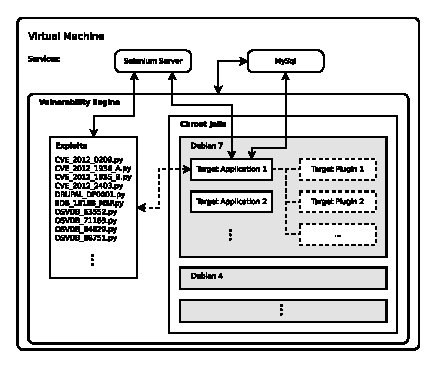
\includegraphics[scale=1.17]{system_diagram.eps}
\end{center}
\caption{System Diagram}
\end{figure}

The major components of the BugBox framework are organized as the Python modules and packages. The system breaks down into the following four modules: {\bf SeleniumDriver}, {\bf Exploit},  {\bf Targets} and {\bf Engine}.  Figure 1 illustrates the general structure of the corpus environment, with arrows showing lines of control or communication. \\  

A corpus entry has three main entities: a script, a trace, and a package.  The script contains the exploit actions that are programmatically taken on a specific application.  This script helps automation and reproducability of results.  The trace is the resultant execution trace of the web application when the script is executed on it.  The trace collected is why we have identified our method as a trace-based collection approach.  The packages represent web applications in their vulnerable state.  Each web application is represented multiple times under different versions, giving accessability to the vulnerable code. 



  Furthermore, the framework capability is streamlined through the thorough use of abstraction and encapsulation making the management of the application, environment, and exploitation in BugBox. 
 The design is intended to make it practical to manage a large database of exploits, along with their target environments while acting as more than an exploit repository through containing the software and its dependencies in which a vulnerability exists, the configuration of the software in it's vulnerable state, exploit code that will trigger the security breach, and data that describes any distinguishing attributes of the bug.

Support that will be effortlessly streamlined because of a scalable framework that is easy to maintain, quick to use, automated, and fully compartmentalized.  




\section{Corpus Entry Workflow}

There are a few simple steps to creating a new corpus entry: determine the exploit, download a package, confirm the exploit, create the script, collect the trace.  As mentioned in the introduction, one could use any vulnerability or exploit database.   Once a particular exploit is found, we verify if the package is available already in the corpus, if not we simply upload it as a new package.  We perform a manual execution of the exploit to verify that we understand the scope of the exploit, from which we proceed to write a script for the exploit so that the process will be automated for future use.  Finally, we collect the trace of the program while our script is being executed and add it to our corpus.



\subsection{Engine}
The {\bf Engine} drives the environment setup, tear-down, and exploitation process.  The engine was created to abstract away details so that contributors can add new exploit scripts without worrying about the setup. The structure of Engine (illustrated in figure 2) is designed so that exploits can be written in a concise code statement.  This separation accomplishs a step-like approach for getting involved with the corpus, where developing exploits for the corpus is more approachable and quick for novice programmers that want to contribute and a robust framework that can be understood incrementally for larger contributions to the framework.  The following is an  example use case for running a script using this engine:
 

\begin{enumerate}
	\item {\tt script.py start}
	\item {\tt script.py xdebug\_on}
	\item {\tt script.py exploit}
	\item {\tt script.py xdebug\_off}
	\item {\tt script.py stop}
\end{enumerate}

During step one the engine creates a chroot environment on the linux distribution for which the target application is copied over and the pertinent MYSQL bindings are established.  The engine can modify the state of the trace collection in X\_Debug as seen in steps two and four to ensure that we collect only the trace pertinent to the exploitation.  Finally, the fifth steps unmounts the chroot environment and returns the corpus environment back to an un-altered state.


\section{Trace Collection}

XDebug is a feature-rich PHP extenstion which provides debugging and profiling cababilities.  For our purposes, we use it to capture traces through setting its global environment auto-trace variable.  Currently we toggle this through the command line, but want future support to be able to toggle the trace collection through the setting of cookies while the script is being executed.


\section{Environment}

We use the linux chroot environment in order to conduct tests in isolation.  Staging the application within the chroot environment provides locality, reproducibility, and stability.\\

{\bf The web application remains local}.  Many applications, such as wordpress, have a MYSQL backend.  If we were to host the application on a different server or VM we would have to ensure that the MYSQL database is properly setup each time.  With the chroot environment, the process is simplified. We keep a MYSQL database outside of the CHROOT Jail in order to facilitate web application configuration.  \\

{\bf Current tests are independent from future tests}.  We load a clean application into the chroot jail every time we wish to run a new test.  This ensures that there is no corruption of the original web application and provides reproducible results when testing.\\

{\bf The web application cannot contaminate our testing environment}.  If a web application crashes due to the malicious script, we can ensure that it does not crash our corpus environment.  In the worst case the chroot becomes corrupt for which we can treat in an isolated scenario tha does not have un-intended side effects in our testing environment.  \\

{\bf The web application will never be contaminated}.  We store a separate backup in order to verify that the selenium scripts did not modify the Web Application in any way.  If the Web Application is corrupt, then we simply copy the web application from the backup folder to the package folder.  Future implementations will store only the md5 hash of the program on the corpus server and the backups on an external server.  This will allow for a quick comparison followed by a remote copy for mismatched hashes.  This separation will ensure that backups will never be corrupted through use of the corpus and expedite checking.  \\

{\bf Applications with different OS environments can be run}.  If an application was built for debian 6 as opposed to debian 4, we can setup a chroot environment that has support for that specific OS.  This gives us the flexibility to test the web application in whatever OS environment we choose.

{\bf Scalability}.  In order to create a system that can handle a growing amount of vulnerabilities that are independent from one another, we represent an exploit on an application through  Selenium scripts, as noted in the Framework section.  Selenium scripts allow us to perform operations on web applications without fear of working in an un-intended, compromised environment.  Scalability is critical because we ultimately want to do mass, automated experiments in tandem. \\


\begin{figure}[!tp]
\begin{center}
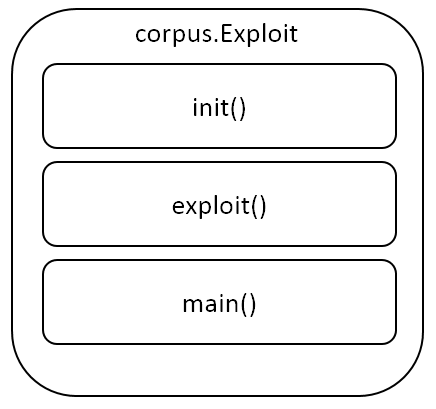
\includegraphics[scale=.5]{Corpus_Exploit.PNG}
\end{center}
\caption{Exploit Structure}
\end{figure}


\subsection{Targets}

   The corpus.{\bf Target} module controls all the application targets that the exploits may be applied to.  More specifically, this represents web applications such as WordPress, SimplePHPAgenda, etc. A copy of the target program with a typical configuration, is always loaded before any exploit script is run.  Init scripts are written per application to provide the corpus.{\bf Engine} with the proper details for the setup, for example:

{\tt \small
\begin{verbatim}
name = "Wordpress 3.3.1"
application_dir_mapping = ...
     [get_path("application"), "/var/www"]
database_filename = get_path("database.sql")
database_name = "wordpress_3_3_1_A"
chroot_environment = "Debian7"
\end{verbatim}
} 


\subsection{Exploit}
The module corpus.{\bf Exploit} is the superclass for each exploit in the corpus, defining interfaces and attributes that the engine uses to manage the environment and exploitation.  This template ensures that the selenium driver is properly bound to the exploit and makes sure that an exploit script has been defined as well as defines any specific actions on teardown.



\subsubsection{init()}

The exploit module is annotated by it's attribute dictionary. This structure is inspired by the exploit class from the Metaploit module. In it we declare the name, description, references, target, type and wiki page for the exploit by the attributes dictionary.  The name is the technical name specified in one of the online databases of exploits and vulnerabilities mentioned earlier in the paper.  The description is a brief statement of what the exploit is supposed to do, because the name is typically not desciptive enough for a person to understand what type of exploit is being applied.  The Target is the web application target that is being used for the exploit.  The type is the type of exploit being conducted.  The VulWikiPage is the wiki page setup for an author to place auxilliary information about the exploit or script.  The following represents an example of a XSS exploit:\\

{\tt \small

\noindent{\bf Name}:	CVE\_2012\_2403\\
{\bf Description}:		Creates a post containing a XSS payload.\\
{\bf References}:	CVE 2012-2403,OSVDB 81463 \\
{\bf Target}: 		Wordpress 3.3.1\\
{\bf Type}: 		XSS\\
{\bf VulWikiPage}: WIKIHOST/CVE-2012-2403

}

\subsubsection{exploit()}

The actual selenium script used for exploitation is contained under the exploit section.  Writing this exploit is as simple as instantiating the selenium driver and submitting a post on the wordpress site with the XSS Payload: 

{\tt \footnotesize
\begin{verbatim}

payload = "XSS PAYLOAD"

driver = self.create_selenium_driver()

driver.get("http://localhost/wordpress/?p=1")
%%Selenium Actions preceded by
% driver.find_element_by_id
("author").clear()
("author").send_keys("selenium script")
("email").clear()
("email").send_keys("selenium@python.org")
("url").clear()
("url").send_keys("www.python.org")
("comment").clear()
("comment").send_keys(payload)
("submit").click()

\end{verbatim}
}

It is important to note that in the creation of this database we will only release exploit scripts that have a patched released for the vulnerability or is properly noted in one of the databases mentioned in the introduction (it does not represent a zero-day exploit.)


\subsection{{\bf SeleniumDriver} and Scripting}
We use the {\bf SeleniumDriver} as a wrapper class for the Selenium's Firefox web driver in order to leverage the Selenium's powerful browser automation.  Selenium integrates nicely with the framework, providing demonstration/visualization capabilities, javascript support, and simple interaction with HTML objects.

\textcolor{red}{To accomplish our trace-based approach, we create a selenium script in Python, replicating actions a user would take in performing an exploit on a web application and collect the execution trace with XDebug.}
We begin the trace-based approach by writing an exploit in Python using Selenium. The exploit script automates all actions an attacker would take in compromising a web application. XDebug is instructed to collect the execution traces during this process, and finally the corpus engine collects and organizes them on a per-session basis.


\section{Lessons Learned}

Some research projects conducted in our software engineering group at the University of Maryland are centered around collection of metrics data for vulnerabilities.  Since we were unable to find a corpus that suited our needs, we started to build an in-house corpus.  Originally we had another VM based architecture in mind. \\

We found that because the process was not documented, it was harder to verify that the exploit was executed in the correct manner.  Many times pages that were logged as exploited, did not show the representation of the exploit.  Furthermore there was no specific collection that could be analyzed of the exploit.\\

We determined that, for one, this environment was not scalable.  We could not continue to add new exploits to a tainted environment without eventually overlapping one exploit with another.  We would have an increasingly hard time to review whether or not an exploit was overlapping.\\

The idea was to be able to mount web application targets onto VMs.  We had a similiar idea in th sense that the VM's could be setup and brought down, saving the current state that they were in.  Once the application was mounted, we performed an exploit manually and saved a snapshot of the VM instance.  All exploits applied to "tainted" applications, so we had to be careful that one exploit did not interfere with another.  We hired summer students to create exploits and save new snapshots, from which we had them report their progress on the wiki we had built.  


\section{Acknowledgements}

Plugs for everyone who has given us money.

\section{Use Cases}
By providing a corpus that explicitly logs the steps taken in accumulating the log files, we have more flexibility.  This flexibility can be seen with the following example:  
\\\\
{\tt Jon is told by his advisor that he needs to collect more trace data in order to get a proper sample size for his research.  John quickly creates a selenium script for the exploit he wants to collect and shows the advisor his results.  The advisor was generally happy with the trace data that he collected, but instead wanted him to do a slight modification to the exploit.  If Jon did not have the selenium script at hand, he would have to duplicate all of the work previously done.  Since he does have the script on hand, he can quickly make a change to the script and re-run in seconds versus hours.}
\\\\
While the above process is only shown in one iteration, most students know that this is not the case.  One hour of work can turn into a whole week of work without the proper framework in place.  The above situation also shows that the selenium script can be discussed with the professor to show validity of the data and provide talking points for how the exploit was applied.


\section{Future Development}
 \begin{description}
   \item[Distribution]
     \textcolor{red}{Virtual machine v.s. debian package. Pre-built chroot jails v.s. build scripts.
     i.e. size <--> setup proceess balance. Striking a balance between}
   \item[Services]
     \textcolor{red}{Why run Selenium/Mysql in VM vs a chroot jail?}
   \item[Isolating attack event]
     \textcolor{red}{(with xdebug manually/cookies/etc...)}   
   \item[Selenium driver and aux modules]
  Future support will control trace collection through cookie manipulation via XDebug. This will reduce the collection of insignificant interactions and provide a more refined break-down of the exploitation process since traces can be grouped by HTML request.  \par
   Explore the possibility of a unified communication interface. This may be necessary in order to cleanly interact with xdebug with appropriate cookies set on a per-request basis (especially when modules other than Selenium are used for communication).
   \item[Payload standardization]
For each exploit currently in the corpus, there is no standard for the payload used in the attack. Since many studies may be sensitive to the payload type and encoding, it makes sense to provide the researcher with fine-grained control over this property. The Metasploit Framework has a very robust system for managing exploits along with their payloads and encodings, and can be a model for implementing this.
 \end{description}


\section{Availability and Use}

BugBox is designed to work with the Debian GNU/Linux distribution and compatible distributions.  It can be distributed as a self-contained virtual machine, or as a package that can be installed on an existing system. The machine must have sufficient storage (roughly 4 GB per OS environment, and 2 GB for the application, engine, and exploit sources [Confirm these \#s]).  Dependencies for BugBox include MySQL,  Selenium Server, debootstrap, and the Advanced Packaging Tool (APT.), and the capacity to run any of the system dependancies of the target web application.

The corpus is publicly available at:

\begin{center}
{\tt git://bugbox.cs.umd.edu/blahblah}
\end{center}

Download scripts, install in box matching requirements section, and exploit in a safe environment.

\begin{center}
{\tt http://www.vulnerabilitywiki.com}
\end{center}

{\footnotesize \bibliographystyle{acm}
\bibliography{ref}}

\end{document}







